\section{光滑三次曲面上的直线}\label{sec:lines-on-smooth-cubic-surfaces}

我们来到本书的最后一节. 本节讨论下面这个经典结果, 它最初由 Arthur Cayley (1821--1895) 和 George Salmon (1819--1904) 于 1849 年证明, 并且建立在我们前面诸多结果的基础上.

\begin{Theorem}{光滑三次曲面上的直线}\leavevmode\label{thm:smooth-cubic-surface-has-twenty-seven-lines}
令 $X\subseteq\mathbb{P}^{3}$ 为一个光滑三次曲面. 则 $X$ 恰好包含 $27$ 条直线.
\end{Theorem}

Theorem~\ref{thm:smooth-cubic-surface-has-twenty-seven-lines} 如此优美的一个原因, 是结论具有一致性: 光滑三次曲面上的直线条数既不依赖于基 (代数闭) 域, 也不依赖于定义它的三次方程. 此外, 光滑二次曲面彼此都射影等价 (Exercise~\ref{ex:smooth-quadric-projectively-equivalent-to-segre-surface}), 光滑三次曲面的情形则不同: 可以证明, 即使计及射影等价, 光滑三次曲面仍有无穷多个彼此不同的例子. 这个无穷族中的每个曲面都有同样多的直线, 十分引人注目! 作为热身, 请读者在 Exercise~\ref{ex:twenty-seven-lines-on-the-fermat-cubic} 中找出 Fermat 三次曲面上的全部 $27$ 条直线. 这是最对称的例子.

一般很难直观地看到 $\mathbb{C}$ 上的三次曲面中的各条直线, 因为复直线通常只在一个点与曲面的实点相交. 然而, $\mathbb{C}$ 上有某些三次曲面, 其所有复直线都包含实直线. 最著名的例子是 Clebsch 三次曲面, 它以 Alfred Clebsch (1833--1872) 命名.

\begin{Example}{Clebsch 三次曲面上的直线}\leavevmode\label{ex:lines-on-clebsch-cubic}
Clebsch 三次曲面定义为
\[
  X=\mathcal{V}(w^{3}+x^{3}+y^{3}+z^{3}-(w+x+y+z)^{3})\subseteq\mathbb{P}^{3}.
\]
下图从三个不同角度画出了 $X$ 的实点的一个仿射限制, 以及 $X$ 上的 $27$ 条直线. 在此仿射限制中, 它们全都能以实直线的形式看到.

\noindent\phantomsection\label{fig:clebsch-cubic-three-views}%
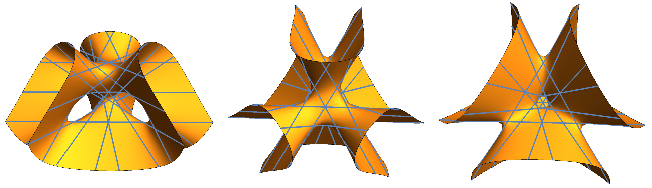
\includegraphics[width=\linewidth]{figures/clebsch-cubic-three-views.pdf}
\end{Example}

为证明 Theorem~\ref{thm:smooth-cubic-surface-has-twenty-seven-lines}, 我们先证明关于光滑三次曲面上直线的若干预备引理. 在整个过程中, 我们反复运用射影等价把直线和平面变换到便于处理的位置, 并注意这些射影等价将光滑三次曲面变为光滑三次曲面. 每一次要说明具有所需性质的射影等价存在时, 都可以把 $\mathbb{P}^{2}$ 和 $\mathbb{P}^{3}$ 中的直线和平面换成 $K^{3}$ 和 $K^{4}$ 中的线性子空间, 从而归结为线性代数的论断; 这些线性代数论证留给读者 (Exercises~\ref{ex:projective-equivalences-of-plane-line-configurations} 和~\ref{ex:projective-equivalences-of-three-space-configurations}).

下面关于光滑三次曲面上直线的引理的证明, 正是利用射影等价简化论证的典型例子.

\begin{Lemma}{在光滑三次曲面上交于一点的直线共面}\leavevmode\label{lem:concurrent-lines-on-smooth-cubic-are-coplanar}
令 $X\subseteq\mathbb{P}^{3}$ 为光滑三次曲面. 若 $X$ 上的直线 $L_{1},L_{2},L_{3}$ 满足 $L_{1}\cap L_{2}\cap L_{3}\ne\varnothing$, 则 $L_{1},L_{2},L_{3}$ 位于同一平面.
\end{Lemma}
\begin{Proof}
假设不可约三次曲面 $X\subseteq\mathbb{P}^{3}$ 包含三条交于一点但不共面的直线; 我们证明 $X$ 在这三条直线的公共交点处奇异.

给定 $\mathbb{P}^{3}$ 中三条交于一点但不共面的直线, Exercise~\ref{ex:projective-equivalences-of-three-space-configurations} 表明, 存在 $\mathbb{P}^{3}$ 的一个射影等价, 将它们送到三条直线 $\mathcal{V}(x,y)$, $\mathcal{V}(x,z)$ 和 $\mathcal{V}(y,z)$, 这三条直线交于点 $[1:0:0:0]$. 因此, 在射影等价的意义下, 可假设 $X$ 包含这三条特定直线. 令 $\mathcal{I}(X)=\langle f\rangle$. 由于 $f$ 在 $\mathcal{V}(x,y)$, $\mathcal{V}(x,z)$ 和 $\mathcal{V}(y,z)$ 上消没, 稍加思考可知, $f$ 的每一项必能被 $x,y,z$ 三个变量中至少两个整除, 因而
\[
  f=xy\ell_{1}+xz\ell_{2}+yz\ell_{3}
  \qquad\text{对某些 }\ell_{1},\ell_{2},\ell_{3}\in K[w,x,y,z]_{1}.
\]
此外, 由不可约性知 $\ell_{1},\ell_{2},\ell_{3}$ 均非零. 计算偏导数, 得
\[
  \begin{aligned}
  \frac{\partial f}{\partial w}
  &=xy\frac{\partial\ell_{1}}{\partial w}+xz\frac{\partial\ell_{2}}{\partial w}+yz\frac{\partial\ell_{3}}{\partial w},\\
  \frac{\partial f}{\partial x}
  &=y\ell_{1}+xy\frac{\partial\ell_{1}}{\partial x}+z\ell_{2}+xz\frac{\partial\ell_{2}}{\partial x}+yz\frac{\partial\ell_{3}}{\partial x},\\
  \frac{\partial f}{\partial y}
  &=x\ell_{1}+xy\frac{\partial\ell_{1}}{\partial y}+xz\frac{\partial\ell_{2}}{\partial y}+z\ell_{3}+yz\frac{\partial\ell_{3}}{\partial y},\\
  \frac{\partial f}{\partial z}
  &=xy\frac{\partial\ell_{1}}{\partial z}+x\ell_{2}+xz\frac{\partial\ell_{2}}{\partial z}+y\ell_{3}+yz\frac{\partial\ell_{3}}{\partial z}.
  \end{aligned}
\]
由于这些偏导数都在 $[1:0:0:0]\in X$ 处消没, 光滑性的 Jacobian 判据 (见 Example~\ref{ex:singularities-of-projective-hypersurfaces}) 蕴含 $X$ 在此点奇异.
\end{Proof}

下一个引理讨论光滑三次曲面与平面相交时可能出现的曲线类型. 作为准备, 回顾任意平面 $P\subseteq\mathbb{P}^{3}$ 都是某个单射的线性映射 $\mathbb{P}^{2}\to\mathbb{P}^{3}$ 的像. 由此, 只需沿这样的单射取原像, 就能将 $P$ 的任一闭子簇视为 $\mathbb{P}^{2}$ 中的射影簇. 此外, 映到同一平面 $P\subseteq\mathbb{P}^{3}$ 的任意两个单射的线性映射 $\mathbb{P}^{2}\to\mathbb{P}^{3}$ 只相差一个 $\mathbb{P}^{2}$ 的射影等价. 由于 $\mathbb{P}^{2}$ 的射影等价保持不可约曲线 $C\subseteq\mathbb{P}^{2}$ 的次数, 因而可谈论平面 $P\subseteq\mathbb{P}^{3}$ 中闭不可约曲线的\textquotedbl{}次数\textquotedbl{}. 有了这一术语, 下面的结果刻画光滑三次曲面与平面相交产生的所有可能的曲线构型.

\begin{Lemma}{光滑三次曲面的线性截面}\leavevmode\label{lem:linear-slices-of-smooth-cubic-surfaces}
令 $X\subseteq\mathbb{P}^{3}$ 为光滑三次曲面, $P\subseteq\mathbb{P}^{3}$ 为平面. 则 $X\cap P$ 恰为下列情形之一:
\begin{enumerate}[label=(\roman*),ref=\roman*]
  \item $P$ 中一条三次不可约曲线,
  \item $P$ 中一条直线与一条二次不可约曲线的并, 或
  \item\label{part:linear-slice-three-distinct-lines} $P$ 中三条不同的直线的并.
\end{enumerate}
\end{Lemma}
\begin{Proof}
令 $X\subseteq\mathbb{P}^{3}$ 为光滑三次曲面, 其中 $\mathcal{I}(X)=\langle f\rangle$, 并令 $P\subseteq\mathbb{P}^{3}$ 为平面. 用射影等价变换 $X$ 和 $P$ 后, 可假定 $P=\mathcal{V}(z)$, 并将 $P$ 与坐标为 $w,x,y$ 的 $\mathbb{P}^{2}$ 等同. $f$ 在 $P$ 上的限制由 $g=f(w,x,y,0)$ 给出, 它是 $K[w,x,y]$ 中的三次齐次多项式. 注意 $g$ 必不为零, 否则 $f$ 就能被 $z$ 整除, 与 $X$ 的不可约性矛盾.

若 $g$ 不可约, 则 $X\cap P$ 是 $P$ 中的一条三次不可约曲线. 若 $g$ 分解为一个线性多项式与一个不可约二次多项式的乘积, 则 $X\cap P$ 为 $P$ 中一条直线与一条二次不可约曲线的并. 为完成证明, 假设 $g$ 分解为三个线性多项式的乘积; 我们必须证明 $X\cap P$ 恰为三条不同的直线的并 (而不是一条或两条直线).

为导出矛盾, 假设 $X\cap P$ 包含的直线少于三条; 我们证明 $X$ 奇异. 由于 $g$ 分解为三个线性多项式的乘积, 但 $\mathcal{V}(g)=X\cap P$ 包含的直线少于三条, $g$ 必有一个重线性因子. 在射影等价的意义下, 可设这个重线性因子消没于直线 $L=\mathcal{V}(y,z)$. 换言之, 对某个非零 $\ell\in K[w,x,y,z]_{1}$, 有 $g=f(w,x,y,0)=y^{2}\ell$, 从而
\[
  f=y^{2}\ell+zq\qquad\text{对某个非零 }q\in K[w,x,y,z]_{2}.
\]
然后计算偏导数即可验证 (Exercise~\ref{ex:repeated-line-in-plane-section-produces-singularity}), 若 $q(a,b,0,0)=0$, 则 $X$ 在点 $[a:b:0:0]\in L$ 处奇异. 由于 $K$ 代数闭, 至少存在一个这样的点. 因此, 若 $X\cap P$ 为不足三条直线的并, 则 $X$ 奇异, 证明完成.
\end{Proof}

\BookPairedNoteLeft{
在 Lemma~\ref{lem:linear-slices-of-smooth-cubic-surfaces} 的情形 (\ref{part:linear-slice-three-distinct-lines}) 中, 三条直线有两种可能的分布: 要么两两相交于 $P$ 中的三个不同点, 要么三条直线相交于 $P$ 中的一个公共点.
}{
给定光滑三次曲面 $X$ 和直线 $L\subseteq X$, 接下来的目标是确定 $X$ 中与 $L$ 相交的所有其他直线. 为此, 研究 $X$ 与所有包含 $L$ 的平面的交. 更确切地说, 若 $P$ 是包含 $L$ 的平面,
}
则由 Lemma~\ref{lem:linear-slices-of-smooth-cubic-surfaces}, $X\cap P$ 或是 $L$ 与一条不可约二次曲线的并, 或还包含 $X$ 上的另外两条直线 (除 $L$ 外). 因为 $X$ 上每条与 $L$ 相交的直线恰好落在后一种平面之一中, 要了解 $X$ 上与 $L$ 相交的直线, 就要刻画哪些包含 $L$ 的平面使 $X\cap P$ 中余下的二次曲线可约. 下一个引理提供了判定一条二次曲线何时可约的计算工具.

\begin{Lemma}{判定二次曲线何时可约}\leavevmode\label{lem:reducibility-criterion-for-conics}
若 $g=ax^{2}+by^{2}+cz^{2}+dxy+exz+fyz\in K[x,y,z]$, 则 $g$ 可约当且仅当
\[
  4abc+def-af^{2}-be^{2}-cd^{2}=0.
\]
\end{Lemma}
\begin{Proof}
设 $K$ 的特征不是 $2$ (特征 $2$ 的情形留给 Exercise~\ref{ex:reducibility-criterion-for-conics-in-characteristic-two}). 给定如引理中的 $g$, 定义矩阵
\[
  M_{g}=\begin{pmatrix}
    2a&d&e\\
    d&2b&f\\
    e&f&2c
  \end{pmatrix}.
\]
注意 $2g$ 可写成矩阵乘积
\[
  2g=(x,y,z)M_{g}(x,y,z)^{T}.
\]
由
\[
  \det(M_{g})=2(4abc+def-af^{2}-be^{2}-cd^{2}),
\]
可见引理中的断言等价于: $g$ 可约当且仅当 $\det(M_{g})=0$.

令 $A=(a_{i,j})$ 为可逆 $3\times3$ 矩阵, 考察多项式 $\tilde g(x,y,z)=g((x,y,z)A^{T})$. 换言之, $\tilde g$ 由 $g$ 经 $A$ 确定的线性变量代换得到:
\[
  \tilde g(x,y,z)=g(a_{1,1}x+a_{1,2}y+a_{1,3}z,\ldots,
  a_{3,1}x+a_{3,2}y+a_{3,3}z).
\]
注意
\[
  2\tilde g=(x,y,z)A^{T}M_{g}A(x,y,z)^{T},
\]
从而有 $M_{\tilde g}=A^{T}M_{g}A$. 由于 $\det(A)=\det(A^{T})\ne0$, 由行列式的乘法性知, $\det(M_{g})=0$ 当且仅当 $\det(M_{\tilde g})=0$. 因此, $\det(M_{g})$ 是否为零, 和 $g$ 的不可约性一样, 在任意可逆线性变量代换下保持不变.

如 Proposition~\ref{prop:irreducible-conics-projectively-equivalent} 的证明所示, 在相差可逆线性变量代换的意义下, 可假设 $g=axy+bxz+cyz$. 只要注意此时 $g$ 可约当且仅当 $a,b,c$ 中有一个为零, 而这又等价于 $\det(M_{g})=2abc=0$, 就得到引理.
\end{Proof}

前两个引理汇成以下结果, 它是计数光滑三次曲面上直线的关键工具.

\begin{Lemma}{光滑三次曲面上的每条直线恰与另外 $10$ 条直线相交}\leavevmode\label{lem:line-on-smooth-cubic-meets-ten-others}
令 $X\subseteq\mathbb{P}^{3}$ 为光滑三次曲面, $L\subseteq X$ 为直线. 则恰好有五个平面 $P$ 包含 $L$, 使 $P\cap L$ 为三条直线的并. 因此, $L$ 与 $X$ 中的另外十条直线相交.
\end{Lemma}
\begin{Proof}
在射影等价的意义下, 可设 $L=\mathcal{V}(y,z)$. 设 $\mathcal{I}(X)=\langle f\rangle$. 由于 $f$ 在 $L$ 上消没, $f$ 的每一项都能被 $y$ 或 $z$ 整除. 按各项关于 $y,z$ 的次数分组, 可写
\begin{equation}\label{eq:cubic-through-line-expanded-in-transverse-variables}
  f=\ell_{1}w^{2}+\ell_{2}wx+\ell_{3}x^{2}+q_{1}w+q_{2}x+c,
\end{equation}
其中 $\ell_{1},\ell_{2},\ell_{3}\in K[y,z]_{1}$ 为线性的, $q_{1},q_{2}\in K[y,z]_{2}$ 为二次的, $c\in K[y,z]_{3}$ 为三次的.

对任意 $a=(a_{0},a_{1})\in K^{2}\setminus\{0\}$, 定义平面 $P_{a}\subseteq\mathbb{P}^{3}$ 为
\[
  P_{a}=\{[\alpha:\beta:a_{0}\gamma:a_{1}\gamma]\mid
  [\alpha:\beta:\gamma]\in\mathbb{P}^{2}\}\subseteq\mathbb{P}^{3}.
\]
注意 $P_{a}$ 包含 $L$ (即 $\gamma=0$ 的部分), 并且 $\mathbb{P}^{3}$ 中包含 $L$ 的每个平面都等于某个 $P_{a}$. 另外, $P_{a}=P_{b}$ 当且仅当对某个 $\lambda\in K\setminus\{0\}$ 有 $a=\lambda b$. 换言之, $\mathbb{P}^{3}$ 中包含 $L$ 的平面与 $\mathbb{P}^{1}$ 中的点一一对应.

用 $t,u,v$ 表示 $P_{a}$ 的定义中 $\mathbb{P}^{2}$ 上的坐标. 在这些坐标下, $f$ 在 $P_{a}$ 上的限制就是 $f^{a}=f(t,u,a_{0}v,a_{1}v)\in K[t,u,v]$, 由 \eqref{eq:cubic-through-line-expanded-in-transverse-variables}, 它等于
\[
  f^{a}=\bigl(\ell_{1}(a)t^{2}+\ell_{2}(a)tu+\ell_{3}(a)u^{2}
  +q_{1}(a)tv+q_{2}(a)uv+c(a)v^{2}\bigr)v.
\]
Lemma~\ref{lem:linear-slices-of-smooth-cubic-surfaces} 蕴含 $X\cap P_{a}$ 为三条直线的并当且仅当 $f^{a}\in K[t,u,v]$ 中的二次因子可约. 由 Lemma~\ref{lem:reducibility-criterion-for-conics}, 这当且仅当
\begin{equation}\label{eq:quintic-of-split-planes-through-cubic-line}
  4\ell_{1}\ell_{3}c+\ell_{2}q_{1}q_{2}-\ell_{1}q_{2}^{2}
  -\ell_{3}q_{1}^{2}-c\ell_{2}^{2}\in K[y,z]
\end{equation}
在 $a$ 处消没. 因此, 为证明引理, 我们必须证明 \eqref{eq:quintic-of-split-planes-through-cubic-line} 在 $\mathbb{P}^{1}$ 中恰有五个零点. 注意 \eqref{eq:quintic-of-split-planes-through-cubic-line} 是 $K[y,z]$ 中的五次齐次多项式, 所以它分解为五个线性多项式, 而我们必须证明这些线性因子互不相同.

设 $a\in\mathbb{P}^{1}$ 是 \eqref{eq:quintic-of-split-planes-through-cubic-line} 的零点, 换言之, $P_{a}\cap X$ 为三条不同直线的并. 在 $\mathbb{P}^{3}$ 的射影等价的意义下, 可假设 $P_{a}=\mathcal{V}(z)$, 等价地, $z$ 是 \eqref{eq:quintic-of-split-planes-through-cubic-line} 的线性因子. 要证明它不是重因子, 必须证明 \eqref{eq:quintic-of-split-planes-through-cubic-line} 不能被 $z^{2}$ 整除. 令 $L_{1},L_{2}$ 为 $X\cap P_{a}$ 中除 $L$ 外的两条直线. 按照 $X\cap P_{a}$ 中三条直线是否有公共交点, 分两种情况.

\textbf{(情形 1: $L\cap L_{1}\cap L_{2}=\varnothing$)} 由于三条直线 $L,L_{1},L_{2}$ 同处于平面 $P_{a}=\mathcal{V}(z)$ 内且没有公共交点, Exercise~\ref{ex:projective-equivalences-of-plane-line-configurations} 蕴含可通过射影等价将这些直线变换为 $L=\mathcal{V}(y,z)$, $L_{1}=\mathcal{V}(w,z)$ 和 $L_{2}=\mathcal{V}(x,z)$. 由于 $f$ 在 $L,L_{1},L_{2}$ 上消没, $f$ 的每一项便能被 $z$ 或 $wxy$ 整除. 从 \eqref{eq:cubic-through-line-expanded-in-transverse-variables} 可知 $z$ 整除 $\ell_{1},\ell_{3},q_{1},q_{2},c$. 由于 $f$ 不可约, $z$ 不整除 $\ell_{2}$. 因此, \eqref{eq:quintic-of-split-planes-through-cubic-line} 中除了最后一项可能例外, 每一项都能被 $z^{2}$ 整除. 要证明 $z^{2}$ 不整除 \eqref{eq:quintic-of-split-planes-through-cubic-line}, 只需证明 $z^{2}$ 不整除三次项 $c$. 最后, 假如 $z^{2}$ 整除 $c$, 则 $X=\mathcal{V}(f)$ 将在 $[0:0:1:0]$ 处奇异. 读者可以用 \eqref{eq:cubic-through-line-expanded-in-transverse-variables} 计算 $f$ 的偏导数, 并利用 $z$ 整除 $q_{1}$ 和 $q_{2}$ 以及 $z^{2}$ 整除 $c$ 来验证. 因此, $X$ 的光滑性蕴含此时 $z$ 不是 \eqref{eq:quintic-of-split-planes-through-cubic-line} 的重线性因子.

\textbf{(情形 2: $L\cap L_{1}\cap L_{2}\ne\varnothing$)} 此时, Exercise~\ref{ex:projective-equivalences-of-plane-line-configurations} 蕴含在射影等价的意义下, 可设 $L=\mathcal{V}(y,z)$, $L_{1}=\mathcal{V}(x,z)$ 和 $L_{2}=\mathcal{V}(x+y,z)$. 因此, $f$ 中不被 $z$ 整除的部分必能被 $xy(x+y)$ 整除. 从 \eqref{eq:cubic-through-line-expanded-in-transverse-variables} 可知 $z$ 整除 $\ell_{1},\ell_{2},q_{1},c$, 并且 $\ell_{3}$ 中 $y$ 的系数与 $q_{2}$ 中 $y^{2}$ 的系数相同. 特别地, 由后一事实可知, $z$ 整除 $\ell_{3}$ 当且仅当 $z$ 整除 $q_{2}$. 由于 $f$ 不可约, $z$ 不能整除两者中的任何一个, 否则 $z$ 将整除 \eqref{eq:cubic-through-line-expanded-in-transverse-variables} 中的每一项. 由于 $z$ 不整除 $q_{2}$, $z^{2}$ 不整除 $\ell_{1}q_{2}^{2}$. 又因 \eqref{eq:quintic-of-split-planes-through-cubic-line} 中的其他各项都能被 $z^{2}$ 整除, 可知 \eqref{eq:quintic-of-split-planes-through-cubic-line} 不能被 $z^{2}$ 整除. 因此, 此时 $z$ 也不是 \eqref{eq:quintic-of-split-planes-through-cubic-line} 的重线性因子.

既然已经验证 \eqref{eq:quintic-of-split-planes-through-cubic-line} 的线性因子各不相同, 便得出它在 $\mathbb{P}^{1}$ 中恰有五个零点, 给出引理陈述中的五个特殊平面. 于是得到引理的最后一个断言: $X$ 上每一条与 $L$ 相交的直线都在唯一一个包含 $L$ 的平面中. 由于 $X$ 与这个平面的交包含两条直线, Lemma~\ref{lem:linear-slices-of-smooth-cubic-surfaces} 蕴含交中一定还有第三条直线. 因此, $X$ 上每条与 $L$ 相交的直线都必在包含 $L$ 的五个特殊平面之一中, 而这样的直线 (除 $L$ 外) 恰有十条.
\end{Proof}

终于可以数出光滑三次曲面上的直线了.

\begingroup
\renewcommand{\AJProofBegin}{%
  \par\addvspace{\topsep}\noindent
  {\sffamily\bfseries\CJKfamily{pffont}Proof of Theorem~\ref{thm:smooth-cubic-surface-has-twenty-seven-lines}}\enspace\ignorespaces
}
\begin{Proof}
令 $X\subseteq\mathbb{P}^{3}$ 为光滑三次曲面, 任选 $X$ 上一条直线 $L_{1}$; 由 Theorem~\ref{thm:cubic-surface-contains-line}, 这样的直线存在. 选择一个平面 $P\subseteq\mathbb{P}^{3}$, 使 $L_{1}\subseteq P$ 且 $X\cap P$ 为三条直线的并; 由 Lemma~\ref{lem:line-on-smooth-cubic-meets-ten-others}, 这样的平面存在. 将这个平面中的另外两条直线记作 $L_{2},L_{3}$. 现在令 $L$ 是 $X$ 上任意一条别的直线. 注意 $L$ 不能位于 $P$ 内, 因为 $X\cap P$ 中仅有 $L_{1},L_{2},L_{3}$ 三条直线. 由于 $\mathbb{P}^{3}$ 中一个平面与不在其中的直线的交是单点, $L\cap P$ 是 $X\cap P=L_{1}\cup L_{2}\cup L_{3}$ 中的一个点. 因此, $L$ 与 $L_{1}\cup L_{2}\cup L_{3}$ 交于唯一一点. Lemma~\ref{lem:concurrent-lines-on-smooth-cubic-are-coplanar} 蕴含该交点不可能是 $L_{1},L_{2},L_{3}$ 中两条或更多直线的交点, 所以 $X$ 上除 $L_{1},L_{2},L_{3}$ 之外的每条直线必须恰好与这三条直线中的一条相交. 由 Lemma~\ref{lem:line-on-smooth-cubic-meets-ten-others}, $X$ 上恰有十条直线与 $L_{1},L_{2},L_{3}$ 中的每一条相交. 又由于每条 $L_{i}$ 都与 $X\cap P$ 中另外两条直线相交, $X$ 中还有八条直线与每条 $L_{i}$ 相交. 由于 $X$ 的每条直线都恰属于上述情况之一, $X$ 包含 $3+8+8+8=27$ 条直线.
\end{Proof}
\endgroup

对任意光滑三次曲面数完直线之后, 最后讨论这些直线相交的组合结构. 引人注目的是, 正如下面将看到的, 哪些直线对相交的组合结构对于每个光滑三次曲面都是一样的. 为了直观呈现哪些直线对相交, 引入光滑三次曲面 $X\subseteq\mathbb{P}^{3}$ 的\emph{直线关联图}: 这是一个 (组合) 图, $X$ 上的每条直线对应一个顶点, 两个顶点之间有边当且仅当相应的两条直线相交. 下一个结果断言此图不依赖于所选的光滑三次曲面 $X$.

\begin{Theorem}{光滑三次曲面上的直线构型}\leavevmode\label{thm:line-incidence-graph-of-smooth-cubic-is-universal}
每个光滑三次曲面都有相同的直线关联图.
\end{Theorem}
\begin{Proof}
令 $G$ 为下图. 我们断言 $G$ 是任意光滑三次曲面的直线关联图. 为此, 设 $X\subseteq\mathbb{P}^{3}$ 是光滑三次曲面; 我们说明怎样用 $X$ 上的直线给 $G$ 的顶点加标记, 使 $G$ 中两个顶点相邻当且仅当对应的两条直线在 $X$ 中相交. 鼓励读者在阅读证明时实际给 $G$ 的各顶点标上记号. 根据所作选择, 给 $G$ 加标记的方法有多种, 这反映了该图的诸多对称性. 首先可检验 $G$ 有 $27$ 个顶点, 代表 $X$ 上的 $27$ 条直线; 每个顶点都与另外 $10$ 个顶点相邻, 这反映了 Lemma~\ref{lem:line-on-smooth-cubic-meets-ten-others} 的结论.

\par\noindent\makebox[\linewidth]{%
  \phantomsection\label{fig:cubic-line-incidence-graph}%
  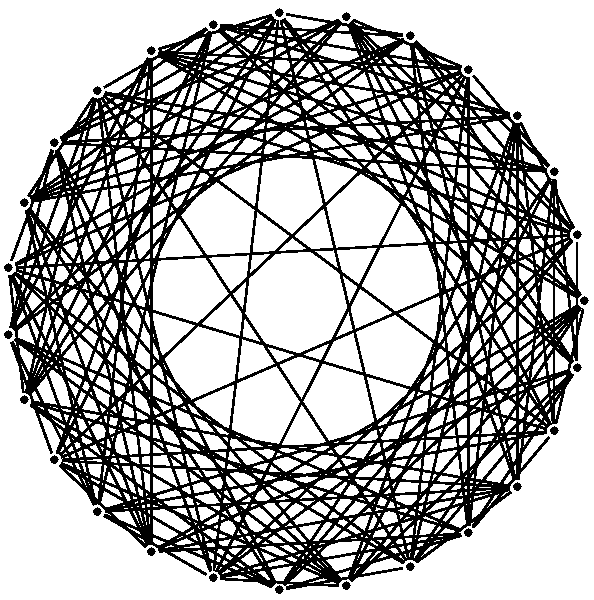
\includegraphics[width=.75\linewidth]{figures/cubic-line-incidence-graph.pdf}%
}

令 $L_{1}\subseteq X$ 为 $X$ 上任意一条直线. (\emph{任选 $G$ 的一个顶点并标记为 $L_{1}$.}) 由于 $L_{1}$ 只与 $X$ 上其余 $26$ 条直线中的十条相交, 存在一条不与 $L_{1}$ 相交的直线 $L'_{1}\subseteq X$. (\emph{任选 $G$ 中不与 $L_{1}$ 相邻的一个顶点并标记为 $L'_{1}$.}) 注意 $L_{1}$ 位于五个特殊平面中, 每个平面都包含 $X$ 上另外两条直线, 且 $L'_{1}$ 恰与每一对这样的直线中的一条相交. 用 $L_{1,2},\ldots,L_{1,6}$ 表示同时与 $L_{1}$ 和 $L'_{1}$ 相交的五条直线. (\emph{找出同时与 $L_{1}$ 和 $L'_{1}$ 相邻的五个顶点, 分别标记为 $L_{1,2},\ldots,L_{1,6}$.}) 由于 $L_{1}$ 与每条 $L_{1,i}$ 相交, 这两条相交直线所确定的平面包含 $X$ 的第三条直线, 记作 $L'_{i}$. (\emph{找出同时与 $L_{1}$ 和 $L_{1,i}$ 相邻的唯一顶点并标记为 $L'_{i}$.}) 类似地, 令 $L_{i}$ 为相交直线 $L'_{1}$ 和 $L_{1,i}$ 所确定的平面中的第三条直线. (\emph{找出同时与 $L'_{1}$ 和 $L_{1,i}$ 相邻的唯一顶点并标记为 $L_{i}$.}) 到此已找到 $X$ 上的 $17$ 条直线:
\[
  L_{1},\ldots,L_{6},L'_{1},\ldots,L'_{6},L_{1,2},\ldots,L_{1,6}.
\]
按构造, 当 $i\ge2$ 时, 形如 $\{L_{1},L_{1,i},L'_{i}\}$ 或 $\{L'_{1},L_{1,i},L_{i}\}$ 的任意三条直线共面, 所以对应顶点在直线关联图中形成三角形. 此外, 对 $1<i<j\le6$, 注意 $L_{i}$ 的选取使它与 $L_{1}$ 不相交, 而且 $L_{i}$ 也与 $L_{1,j}$ 不相交. 否则, 它必须与相交的两条直线 $L_{1,j}$ 和 $L'_{1}$ 同处一个平面, 但已知该平面中的第三条直线是 $L_{j}\ne L_{i}$. 因为 $L_{i}$ 既不与 $L_{1}$ 相交也不与 $L_{1,j}$ 相交, 所以 $L_{i}$ 必与它们所确定的平面中的第三条直线 $L'_{j}$ 相交. 类似地, 对 $1<i<j\le6$, 直线 $L'_{i}$ 与 $L_{j}$ 相交. 因此, 对所有不同的 $i,j\in\{1,\ldots,6\}$, 对应于直线对 $\{L_{i},L'_{j}\}$ 的顶点在 $X$ 的直线关联图中相邻. 本段所述直线关联图中的 $50$ 条边, 对应于 $G$ 中连接迄今已标记的 $17$ 个顶点的全部边, 读者易于验证.

对每个 $1<i<j\le6$, 注意此前找到的 $17$ 条直线中没有一条同时与两条相交的直线 $L_{i}$ 和 $L'_{j}$ 相交. 所以, $L_{i}$ 和 $L'_{j}$ 所确定的平面上的第三条直线还不在清单中, 将其记作 $L_{i,j}$. (\emph{找出同时与 $L_{i}$ 和 $L'_{j}$ 相邻的唯一顶点并标记为 $L_{i,j}$.}) 由于这样的新直线有 $10$ 条, 现在已找齐 $X$ 上的全部 $27$ 条直线. 对 $1<i<j\le6$, $L_{i,j}$ 与 $L_{1}$ 不相交, 因为与 $L_{1}$ 相交的 $10$ 条直线已全部列出. 而且 $L_{i,j}$ 与 $L_{1,i}$ 也不相交, 因为它与 $\{L'_{1},L_{1,i},L_{i}\}$ 三条直线中的另一条相交. 因此, $L_{i,j}$ 必与 $\{L_{1},L_{1,i},L'_{i}\}$ 三条直线中的 $L'_{i}$ 相交. 同理, $L_{i,j}$ 必与 $L_{j}$ 相交. 这样, 在直线关联图中, 对应于 $\{L_{i,j},L_{i}\}$, $\{L_{i,j},L'_{i}\}$, $\{L_{i,j},L_{j}\}$ 和 $\{L_{i,j},L'_{j}\}$ 各对直线的顶点都相邻, 得到直线关联图中另外 $40$ 条边.

至此已经列出了与任意 $L_{i}$ 或 $L'_{i}$ 相交的全部 $10$ 条直线, 只剩下描述哪些形如 $L_{i,j}$ 的直线彼此相交. 若 $i,j,k,\ell$ 各不相同, 由于 $L_{i,j}$ 既不与 $L_{k}$ 相交也不与 $L'_{\ell}$ 相交, 它必与 $\{L_{k},L_{k,\ell},L'_{\ell}\}$ 三条直线中的 $L_{k,\ell}$ 相交. 因此, 只要 $\{i,j\}\cap\{k,\ell\}=\varnothing$, $L_{i,j}$ 就与 $L_{k,\ell}$ 相交, 得到直线关联图中另外 $45$ 条边. 由于已描述了每个 $L_{i,j}$ 的 $10$ 个相邻顶点, 可以断定已经找齐 $X$ 的直线关联图中所有可能的边.

总之, $X$ 上的 $27$ 条直线可以分成六条彼此不相交的直线 $L_{1},\ldots,L_{6}$, 六条彼此不相交的直线 $L'_{1},\ldots,L'_{6}$, 以及 $15$ 条直线 $L_{i,j}$, 其中 $1\le i<j\le6$, 且
\begin{itemize}
  \item $L_{i}$ 与 $L'_{j}$ 相交当且仅当 $i\ne j$,
  \item $L_{i}$ 与 $L_{j,k}$ 相交当且仅当 $i\in\{j,k\}$,
  \item $L'_{i}$ 与 $L_{j,k}$ 相交当且仅当 $i\in\{j,k\}$, 并且
  \item $L_{i,j}$ 与 $L_{k,\ell}$ 相交当且仅当 $\{i,j\}\cap\{k,\ell\}=\varnothing$.
\end{itemize}
请读者核对, 这些相交关系都与按照自己标记的图 $G$ 中的 $135$ 条边一致.
\end{Proof}

\leavevmode\phantomsection\label{idx:eckardt-point}虽然 Theorem~\ref{thm:line-incidence-graph-of-smooth-cubic-is-universal} 表明每个光滑三次曲面的直线关联图都相同, 但最后指出, 直线相交的组合结构并非对所有光滑三次曲面都完全一致. 特别地, 三次曲面上的\emph{Eckardt 点}是该曲面上三条直线的公共交点. 某些特殊三次曲面有 Eckardt 点 (例如, Example~\ref{ex:lines-on-clebsch-cubic} 的图表明 Clebsch 曲面有这样的点, 而 Exercise~\ref{ex:twenty-seven-lines-on-the-fermat-cubic} 表明 Fermat 三次曲面也有), 但一般的三次曲面没有 Eckardt 点.

\BookExerciseHeading
\begin{BookExercises}
  \item\label{ex:twenty-seven-lines-on-the-fermat-cubic} 令 $X=\mathcal{V}(x_{0}^{3}+x_{1}^{3}+x_{2}^{3}+x_{3}^{3})\subseteq\mathbb{P}^{3}$ 为 Fermat 三次曲面.
  \begin{enumerate}
    \item 证明 $X$ 光滑.
    \item 给出 $X$ 上每条直线的参数化, 共 $27$ 条.
    \item 令 $\zeta$ 为一个三次单位根, 并设 $0\le i<j\le3$. 证明平面 $\mathcal{V}(x_{i}+\zeta x_{j})$ 包含 $X$ 上三条直线, 且这三条直线的交非空.
    \item 找出 $X$ 上的 $18$ 个点, 使 $X$ 上的三条直线在每个这样的点相交.
  \end{enumerate}
  \item\label{ex:projective-equivalences-of-plane-line-configurations} 证明对下列每项, 都存在满足所述性质的 $\mathbb{P}^{2}$ 的射影等价.
  \begin{enumerate}
    \item 将任意直线 $L$ 送到直线 $\mathcal{V}(x)$.
    \item 将任意一对直线 $L_{1},L_{2}$ 送到直线 $\mathcal{V}(x),\mathcal{V}(y)$.
    \item 将满足 $L_{1}\cap L_{2}\cap L_{3}=\varnothing$ 的任意三条直线 $L_{1},L_{2},L_{3}$ 送到直线 $\mathcal{V}(x),\mathcal{V}(y),\mathcal{V}(z)$.
    \item 将满足 $L_{1}\cap L_{2}\cap L_{3}\ne\varnothing$ 的任意三条直线 $L_{1},L_{2},L_{3}$ 送到直线 $\mathcal{V}(x),\mathcal{V}(y),\mathcal{V}(x+y)$.
  \end{enumerate}
  \item\label{ex:projective-equivalences-of-three-space-configurations} 证明对下列每项, 都存在满足所述性质的 $\mathbb{P}^{3}$ 的射影等价.
  \begin{enumerate}
    \item 将任意直线 $L$ 送到直线 $\mathcal{V}(y,z)$.
    \item 将任意平面 $P$ 送到平面 $\mathcal{V}(z)$.
    \item 将满足 $L_{1}\cap L_{2}\cap L_{3}\ne\varnothing$ 的任意三条不共面直线 $L_{1},L_{2},L_{3}$ 送到直线 $\mathcal{V}(x,y)$, $\mathcal{V}(x,z)$, $\mathcal{V}(y,z)$.
  \end{enumerate}
  \item\label{ex:repeated-line-in-plane-section-produces-singularity} 设 $f$ 为形如 $f=y^{2}\ell+zq$ 的不可约多项式, 其中 $\ell$ 和 $q$ 分别是 $K[w,x,y,z]_{1}$ 和 $K[w,x,y,z]_{2}$ 中的非零元素. 证明若 $q(a,b,0,0)=0$, 则 $\mathcal{V}(f)\subseteq\mathbb{P}^{3}$ 在点 $[a:b:0:0]$ 处奇异.
  \item\label{ex:reducibility-criterion-for-conics-in-characteristic-two} 设 $K$ 的特征为 $2$, 并考察齐次二次多项式 $g=ax^{2}+by^{2}+cz^{2}+dxy+exz+fyz\in K[x,y,z]$. 证明 $g$ 可约当且仅当 $def-af^{2}-be^{2}-cd^{2}=0$.
  \item\label{ex:smooth-quadric-iff-doubly-ruled} 令 $X\subseteq\mathbb{P}^{3}$ 为二次曲面.
  \begin{enumerate}
    \item 设 $X$ 光滑. 证明 $X$ 的每一点恰好包含于 $X$ 上的两条直线中.
    \item 设 $X$ 中某一点仅包含于 $X$ 上的一条直线中. 证明 $X$ 奇异.
    \item 设 $X$ 中某一点包含于 $X$ 上两条以上直线中. 证明 $X$ 奇异.
  \end{enumerate}
  \item\label{ex:smooth-quadric-projectively-equivalent-to-segre-surface} 令 $X\subseteq\mathbb{P}^{3}$ 为光滑二次曲面.
  \begin{enumerate}
    \item 证明 $X$ 包含三条彼此不相交的直线.
    \item 证明 $\mathbb{P}^{3}$ 中任意三条彼此不相交的直线与三条直线 $\mathcal{V}(w,x),\mathcal{V}(y,z),\mathcal{V}(w-y,x-z)$ 射影等价.
    \item 证明 $X$ 与 $\mathcal{V}(wz-xy)\subseteq\mathbb{P}^{3}$ 射影等价.
  \end{enumerate}
\end{BookExercises}
